
\subsection{Principe}
 Nous cherchons dans cette partie à exprimer une fonction passant (ou approchant) par chaque point de notre tableau expérimental. Le tableur utilisé dans ce projet (LibreOffice) ne possède pas de fonctions d'interpolation automatique pour un polynôme de degré défini.
 Nous avons alors cherché ``à la main'' cette fonction en utilisant la méthode suivante: \vspace{1cm}\\
 
 D'après l'étude théorique de la partie \ref{c_theorique}, nous connaissons le rang maximum de la fonction. Par exemple, pour l'algorithme $A_1$, nous sommes en recherche d'une forme $\alpha x^3 + \beta x^2 + \Gamma x + c$.\\
 Pour retrouver ces différents coefficients, nous avons utilisé cet algorithme :
 \begin{itemize}
  \item Augmenter $\alpha$ jusqu'à ce que les valeurs de $f(x)$ approchent des valeurs expérimentales sans les dépasser.
  \item Augmenter $\beta$ de la même manière en conservant $\alpha$ comme acquis.
  \item Réitérer pour les coefficients suivants.
 \end{itemize}
Coefficient après coefficient, nous affinons ainsi la fonction afin qu'elle approche au maximum des points connus. La pertinence de cette méthode repose essentiellement sur la qualité des mesures effectuées. En outre, si une mesure est beaucoup plus faible que la normale, notre méthode ne corrigera pas ce défaut et amplifiera les écarts par la suite.\\
Une réflexion plus approfondie nous aurait permis de traiter ces erreurs en calculant systématiquement les écarts à la courbe et en minimisant ces valeurs.
\subsection{Résultats}
\begin{figure}[p]
  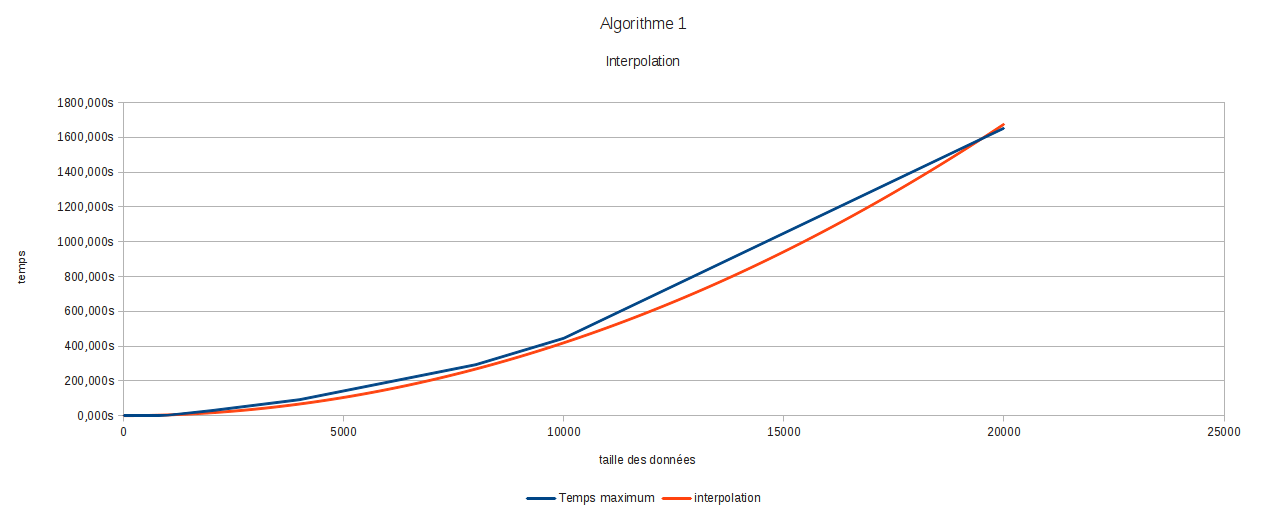
\includegraphics[width=\textwidth]{interpo_algo1}
  \caption{Interpolation de l'algorithme 1}
    \label{interpo1}
\end{figure}
\begin{figure}[p]
  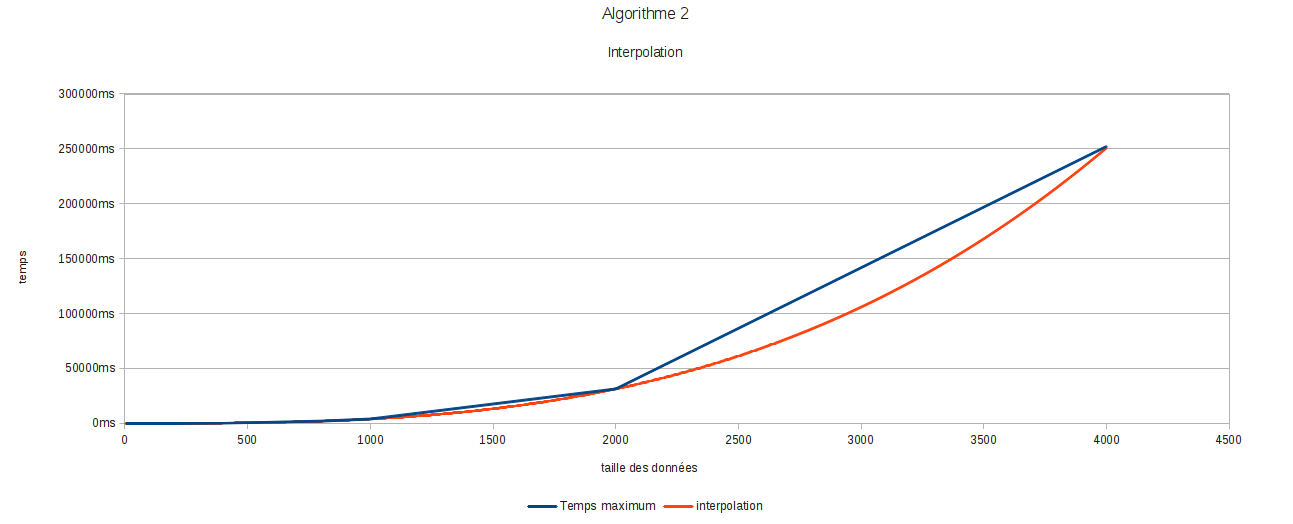
\includegraphics[width=\textwidth]{interpo_algo2}
  \caption{Interpolation de l'algorithme 2}
    \label{interpo2}
\end{figure}
\begin{figure}[p]
  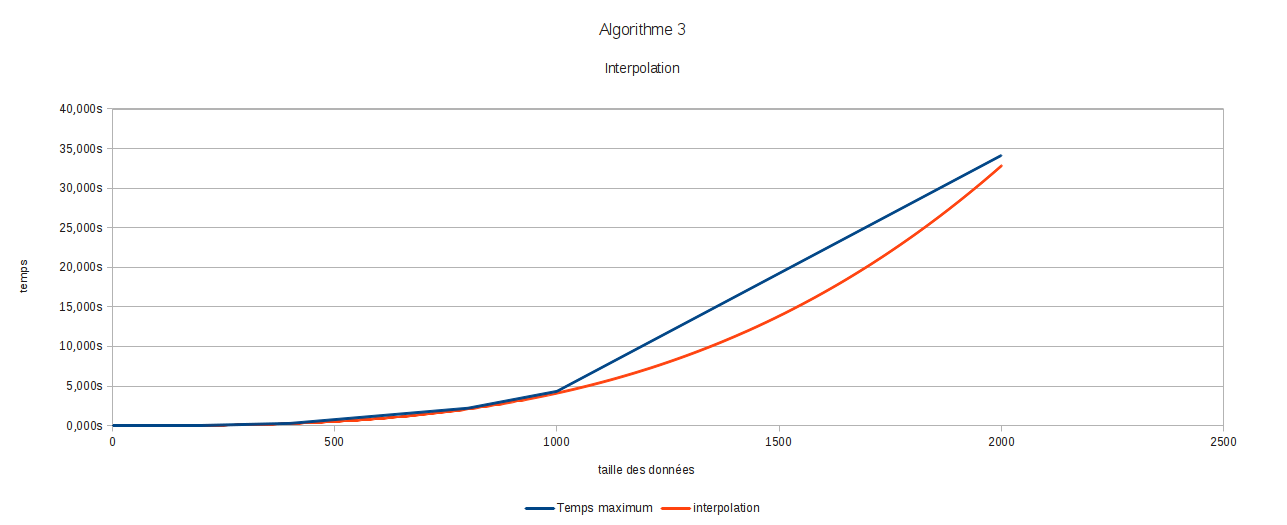
\includegraphics[width=\textwidth]{interpo_algo3}
  \caption{Interpolation de l'algorithme 3}
    \label{interpo3}
\end{figure}

Par la méthode d'approche décrite ci-dessus, nous obtenons pour les trois algorithmes les équations suivantes :
\begin{itemize}
 \item $f_{A_1}(x)=4.09\times 10^{-6} x^2 + 10^{-4}x$ ce qui revient à une complexité en $O(n^2)$ 
 \item $f_{A_2}(x)=3.92\times 10^{-9}x^3 + 10^{-9} x^2 + 5\times 10^{-6} x$ ce qui revient à une complexité en $O(n^3)$ 
  \item $f_{A_3}(x)=4.1\times 10^{-9}x^3 + 10^{-10} x^2 + 3\times 10^{-6} x$ ce qui revient à une complexité en $O(n^3)$ 
\end{itemize}

Les figures \ref{interpo1} \ref{interpo2} et \ref{interpo3} représentent le tracé de la fonction obtenue et leurs comparaison avec la courbe expérimentale de coût au pire pour les trois algorithmes.\\
Les coefficients sont de l'ordre de $10^{-6}$, ce qui s'explique par la puissance actuelle des processeurs, dont la fréquence est de l'ordre de $10^9Hz$. Pour les algorithmes $A_1$ et $A_3$, on retrouve les degrés maximum calculés dans la section \ref{c_theorique}.\\
En revanche, notre ``interpolation'' à partir des résultats de $A_2$ nous donne une fonction en $O(n^3)$ au lieu de $O(n^4)$. Cela peut s'expliquer par un coefficient très faible associé au degré 4 de l'équation réelle. 
Le faible nombre de points dans le tableau nous a permis d'approcher une fonction en $O(n^2)$ probablement invalide pour des valeurs supérieures. De même, l'écart entre la courbe théorique et la courbe extrapolée démontre que notre choix des coefficients n'est pas optimal pour de grandes valeurs.